\documentclass[12pt, oneside]{article}
\usepackage{graphicx}
\usepackage{url}
\usepackage{natbib} 
\usepackage{framed}
\graphicspath{{./BW/}}
%\graphicspath{{./Color/}}

\oddsidemargin 0.1in \topmargin -0.5in \textwidth 6.3in \textheight 9.in

\begin{document}
\title{Predicting the Present with Google Trends}
\author{Hyunyoung Choi, $~$ Hal Varian\footnote{hal@google.com}} 
\date{\today}

\maketitle
\begin{abstract}\noindent In this paper we show how to use search
  engine data to forecast near-term values of economic indicators. Examples
  include automobile sales, unemployment claims, travel destination
  planning, and consumer confidence.
\end{abstract}

\noindent Government agencies periodically release indicators of the
level of economic activity in various sectors.  However, these
releases are typically only available with a reporting lag of several
weeks and are often revised a few months later.  It would clearly be
helpful to have more timely forecasts of these economic indicators.

% \footnote{See, for example, the
% Federal Reserve Economic Data (FRED) available at
% \url{htt://research.stlouisfed.org/fred2/}.}

Nowadays there are several sources of data on real-time economic
activity available from private sector companies such as Google,
MasterCard, Federal Express, UPS, Intuit and many others.  In this
paper we examine Google Trends, which is a a real-time daily and
weekly index of the volume of queries that users enter into Google.
We have found that these query indices are often correlated with
various economic indicators and may be helpful for short-term economic
prediction.

We are not claiming that Google Trends data can help in {\it
  predicting the future.\/} Rather we are claiming that Google Trends
may help in {\it predicting the present.}  For example, the volume of
queries on automobile sales during the second week in June may be
helpful in predicting the June auto sales report which is 
released several weeks later in July.

It may also be true that June queries help to predict July sales, but
we leave that question for future research, as this depends very much
on the particular time series in question.  We have found that queries
{\it can\/} be useful leading indicators for subsequent consumer
purchases in situations where consumers start planning purchases
significantly in advance of their actual purchase decision.

Predicting the present, in the sense described above, is a form of
``contemporaneous forecasting'' or ``nowcasting,'' a topic which is of
particular interest to central banks and other government agencies.
As \cite{Castle09} point out, contemporaneous forecasting is valuable
in itself, but it also raises a number of interesting econometric
research questions involving topics such as variable selection, mixed
frequency estimation, and incorporation of data revisions, to name
just a few.

Our goals in this paper are to familiarize readers with Google Trends
data, illustrate some simple forecasting methods that use this data,
and encourage readers to undertake their own analyses.

We do not claim any methodological advances here; certainly it is
possible to build more sophisticated forecasting models than those we
use.  However, we believe that the models we describe can serve as
baselines to help analysts get started with their own modeling efforts
and that can subsequently be refined for specific
applications.\footnote{This paper is a much simplified and streamlined
  version of our earlier working papers, \cite{Choi09a,Choi09b} which
  includes other more sophisticated models.}

Our examples use {\tt R}, a freely available open-source statistics
package from \url{http://CRAN.R-project.org}.  We provide the {\tt R}
source code and data in the online appendix available at \url{http:to
  be provided}.

\section{Literature review}

So far as we know, the first published paper that suggested that web
search data was useful in forecasting economic statistics was
\citet{Ettredge05}, which examined the U.S. unemployment rate.  At
about the same time \citet{Cooper05} described using internet search
volume for cancer-related topics.  Since then there have been several
papers that have examined web search data in various fields.

For example, in the field of epidemiology, \citet{Polgreen08} and
\citet{Ginsberg09} showed that search data could help predict the
incidence of influenza-like diseases.  This work was widely publicized
and stimulated several further findings in epidemiology, including
\citet{Brownstein09}, \citet{Corley09}, \citet{Hulth09},
\citet{Turbelin09}, \citet{Valdivia10}, and \citet{Wilson09}.

In economics, \citet{Choi09a, Choi09b} described how to use Google
Search Insights data to predict several economic metrics including
initial claims for unemployment, automobile demand, and vacation
destinations; this report is an updated and streamlined version of
those working papers.  \citet{Askitas10}, \citet{Damuri10},
and \citet{Suhoy09} examined unemployment in the US, Germany
and Israel.  \citet{Guzman11} has examined Google data as a predictor
of inflation.

Recently, \citet{Baker11} have used Google search data to examine how
job search responded to extensions of unemployment payments.

\citet{Radinsky09}, \citet{Huang10}, and \citet{Preis10} examine the
use of search data for measuring consumer sentiment while
\citet{Schmidt09} and \citet{Lindberg11} examine retail sales and
consumption metrics.  \citet{Wu10} examine housing data using
longitudinal data extracted from Google Search Insights.

\citet{Shimshoni10} describe the predictability of Google Trends data
itself, pointing out that a substantial amount of search terms are
highly predictable using simple seasonal decomposition methods.

\citet{Goel10} provide a useful survey of work in this area and
describe some of the limitations of web search data.  As they point
out, search data is easy to acquire and is often helpful in making
forecasts, but may not provide dramatic increases in
predictability.  Although we generally agree with this view, we
typically find economically significant, if not dramatic, improvements
in forecast performance using search engine data, as illustrated in
this paper.

Finally, \citet{BOE11} summarize how web search data can be used for
economic nowcasting by central banks.

\section{Google Trends\label{trends}}  
\pagenumbering{arabic}

Google Trends provides a time series index of the volume of queries
users enter into Google in a given geographic area.

The query index is based on {\it query share}: the total query volume
for the search term in question within a particular geographic region
divided by the total number of queries in that region during the time
period being examined.  The maximum query share in the time period
specified is normalized to be 100 and the query share at the initial
date being examined is normalized to be zero.  

The queries are ``broad matched'' in the sense that queries such as
[used automobiles] are counted in the calculation of the query index
for [automobile].  The data go back to January 1, 2004.

Note that Google Trends data is computed using a sampling method and
the results therefore vary a few percent from day to day.
Furthermore, due to privacy considerations, only queries with a
meaningful volume are tracked.  There is a substantial amount of
online help available via links on the site which describe details of
how of how the data is collected.

This query index data is available at country, state, and metro level
for the United States and several other countries. There are two user
interfaces for the data, Google Trends and Google Insights for Search
(I4S).  The latter is the more useful for our purposes since it allows
a logged-in user to download the query index data as a CSV file.

Figure \ref{Fig:free-shipping} depicts example output from I4S for the
query [free shipping] in Australia. The search share for this query
has exhibited significant increase since 2008 and tends to peak during
the holiday shopping season.

\begin{figure}[ht]
\begin{center}
\includegraphics[width=5.2in]{free-shipping}
\caption{\label{Fig:free-shipping} Search index for [free shipping] in
Australia} 
\end{center}
\end{figure}

Google classifies search queries into about 30 categories at the top
level and about 250 categories at the second level using a natural
language classification engine.  For example, the query [car tire]
would be assigned to category {\tt Vehicle Tires} which is a
subcategory of {\tt Auto Parts} which is a subcategory of {\tt
  Automotive.}  The assignment is probabilistic in the sense that a
query such as [apple] could be partially assigned to {\tt Computers \&
  Electronics}, {\tt Food \& Drink}, and {\tt Entertainment}. 

\section{Examples}

\subsection{Motor vehicles and parts}
As an initial example we use the ``Motor Vehicles and Parts Dealers''
series from the U.S. Census Bureau ``Advance Monthly Sales for Retail
and Food Services'' report.\footnote{\url{http://www.census.gov/retail/marts/www/timeseries.html}.}

This index summarizes results from a survey sent to motor vehicle and
parts dealers that asks about current sales.  The preliminary index is
released 2 weeks after the end of each month.  The data is available
in both seasonally adjusted and unadjusted form; here we use the
unadjusted data.  

Let $y_t$ be the log of the observation at time $t$.  We first
estimate a simple baseline seasonal AR-1 model $y_t = b_1y_{t-1} +
b_{12} y_{t-12} + e_t$ for the period 2004-01-01 to 2011-07-01.
%\begin{framed}
\small
\begin{verbatim}
              Estimate Std. Error t value Pr(>|t|)    
  (Intercept)  0.67266    0.76355   0.881 0.381117    
  lag(y, -1)   0.64345    0.07332   8.776 3.59e-13 ***
  lag(y, -12)  0.29565    0.07282   4.060 0.000118 ***
  ---
  Multiple R-squared: 0.7185,	Adjusted R-squared: 0.7111 
\end{verbatim}
%\end{framed}
\normalsize

Google Trends contains several automotive-related categories.  We use
the searches from the first Sunday-Saturday contained in the month,
which gives us a 4-6 week forecasting lead.  A little experimentation
shows that two of these categories, {\tt Trucks \& SUVs} and {\tt
  Automotive Insurance} significantly improve in-sample fit when added
to this regression.

%\begin{framed}
\small
\begin{verbatim}
              Estimate Std. Error t value Pr(>|t|)    
  (Intercept) -0.45798    0.78438  -0.584 0.561081    
  lag(y, -1)   0.61947    0.06318   9.805 5.09e-15 ***
  lag(y, -12)  0.42865    0.06535   6.559 6.45e-09 ***
  suvs         1.05721    0.16686   6.336 1.66e-08 ***
  insurance   -0.52966    0.15206  -3.483 0.000835 ***
  ---
  Multiple R-squared: 0.8179,	Adjusted R-squared: 0.808 
\end{verbatim}
%\end{framed}
\normalsize

However, the perils of in-sample forecasting are well-known.  The
question of interest is whether the Trends variables improve
{\it out-of-sample forecasting.}

To check this, we use a rolling window forecast where we estimate the
model using the data for periods $k$ through $t-1$ and then forecast
$y_t$ using $y_{t-1}$, $y_{t-12}$, and the {\it contemporaneous\/}
values of the Trends variables as predictors.  Since the series is
actually released 2 weeks after the end of each month, this gives us a
meaningful forecasting lead.  The value of $k$ is chosen so that there
are a reasonable number of observations for the first regression in
the sequence.  In this case we chose $k=17$, which implied the
forecasts start in 2005-06-01.

The results are shown in Figure \ref{Fig:autos}.  The mean absolute
error of log$(y_t)$ using the baseline seasonal AR-1 model is 6.34\%
while the MAE using the Trends data is 5.66\%, an improvement of
10.6\%.  If we look at the MAE during the recession (December 2007
through June 2009) we find that the MAE without Trends data is 8.86\%
and with Trends data is 6.96\%, an improvement of 21.4\%.

\begin{figure}[ht]
\begin{center}
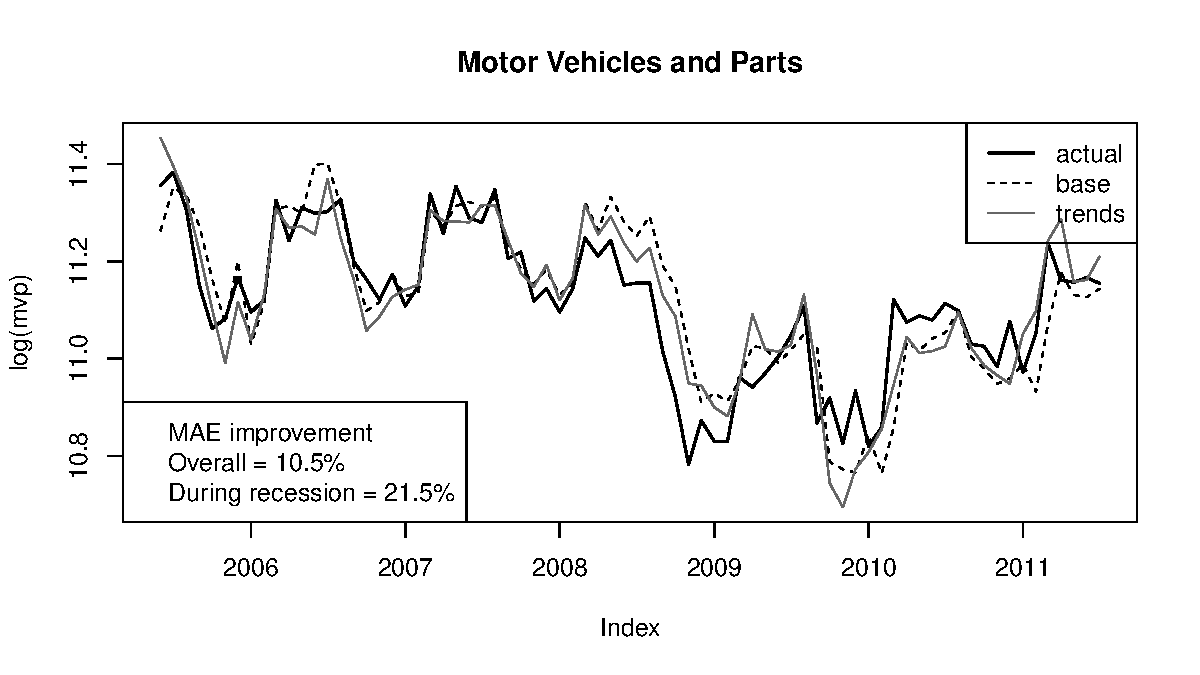
\includegraphics[width= 5.5in]{autos}
\caption{\label{Fig:autos} Motor Vehicles and Parts} 
\end{center}
\end{figure}

\subsection{Initial claims for unemployment benefits}
Each Thursday morning the US Department of Labor releases a report
describing the number of people who filed for unemployment benefits in
the previous
week.\footnote{\url{http://www.dol.gov/opa/media/press/eta/ui/current.htm}}

Initial claims have a good record as a leading
indicator. Macroeconomist Robert Gordon indicates that there is a
``surprisingly tight historical relationship in past US recessions
between the cyclical peak in new claims for unemployment insurance
(measured as a four-week moving average) and the subsequent NBER
trough."\footnote{See \url{http://www.voxeu.org/index.php?q=node/3524}
  for details} Furthermore, a cursory inspection of relationship
between initial claims and the unemployment rate indicates that
initial claims tend to peak 12--18 months before the unemployment rate
peaks.

When someone becomes unemployed it is natural to expect that they will
issue searches such as [file for unemployment], [unemployment office],
[unemployment benefits], [unemployment claim], [jobs], [resume] and so
on. Google Trends classifies search queries like these into two
categories, {\tt Local/Jobs} and {\tt Society/Social Services/Welfare \&
Unemployment}.

In this example we work with the seasonally adjusted initial claims
data, since that is the number used by most economic forecasters.
Since our dependent variable is seasonally adjusted, it makes sense to
seasonally adjust the independent variables as well, so we used the {\tt
  stl} command in {\tt R} to remove the seasonal component of the
Trends data.  

In this case, our baseline regression is a simple AR-1 model on the log
of initial claims.

%\begin{framed}
\small
\begin{verbatim}
Start = 2004-01-17, End = 2011-07-02
              Estimate Std. Error t value Pr(>|t|)    
  (Intercept)  0.25488    0.12951   1.968   0.0498 *  
  L(y, 1)      0.98022    0.01007  97.368   <2e-16 ***
  ---
  Multiple R-squared: 0.9607,	Adjusted R-squared: 0.9606 
\end{verbatim}
%\end{framed}
\normalsize

Note that the coefficient on the lagged term is almost 1 suggesting
that the process for initial claims is very close to a random walk
(with drift).

As \cite{Nelson82} and many subsequent authors have pointed out, it is
very common for macroeconomic data to be represented as a random walk.
For a random walk, the best univariate forecast for $y_t$ is simply
$y_{t-1}$.  However, perhaps we can improve on this baseline forecast
by using additional predictors from Google Trends.

Using the Google Trends categories {\tt Jobs} and {\tt
  Welfare...Unemployment} we find that these are marginally
significant but have little impact on in-sample fit.

%\begin{framed}
\small
\begin{verbatim}
                          Estimate Std. Error t value Pr(>|t|)    
  (Intercept)            1.0563440  0.2686360   3.932 9.98e-05 ***
  L(y, 1)                0.9183560  0.0208778  43.987  < 2e-16 ***
  Jobs                   0.0007069  0.0003847   1.838   0.0669 .  
  Welfare...Unemployment 0.0003752  0.0001838   2.042   0.0418 *  
  ---
  Multiple R-squared: 0.962,	Adjusted R-squared: 0.9618 
\end{verbatim}
%\end{framed}
\normalsize

When we look at one-step-ahead out-of-sample forecasts we find that
the MAE goes from 3.37\% using the baseline forecast to 3.68\% using
the Trends data which is a 5.95\% {\it reduction\/} in fit.  However,
when we look at the series a bit more closely a rather different
picture emerges.

It is well-known that it is difficult to identify ``turning points''
in economic series.  A smoothly increasing or decreasing trend is easy
to fit with a simple linear AR model.  Turning points in time series
are much harder to forecast.

If we look just at the recession period (December 2007 through June
2009) we find that using Trends data reduces the MAE from 3.98\% to
3.44\%, an improvement of 13.6\%.  Looking more closely at the series,
we see that there are four notable turning points indicated by the
shaded areas in Figure \ref{Fig:iclaims}.  The MAE for the period
surrounding these turning points are reported in Table
\ref{Tab:iclaims}. Note that there is a reduction in MAE at all
turning points, with particularly pronounced reductions in the first
two.  In this case, the Google Trends data seems to help in identifying at
least two of the turning points in the series.


\bigskip
\begin{table}
\begin{center}
\begin{tabular}{ r r r r r }
start & end & MAE base & MAE trends & 1-ratio \\
\hline
2009-03-01&2009-05-01&0.0306&0.02398&21.85\% \\
2009-12-01&2010-02-01&0.0356&0.03127&12.36\% \\
2010-07-15&2010-07-15&0.0513&0.05101& 0.65\% \\
2011-01-01&2011-05-01&0.0252&0.02446& 3.22\% \\
\hline
\end{tabular}
\end{center}
\caption{Behavior of MAE around turning points.\label{Tab:iclaims}}
\end{table}


\begin{figure}[ht]
\begin{center}
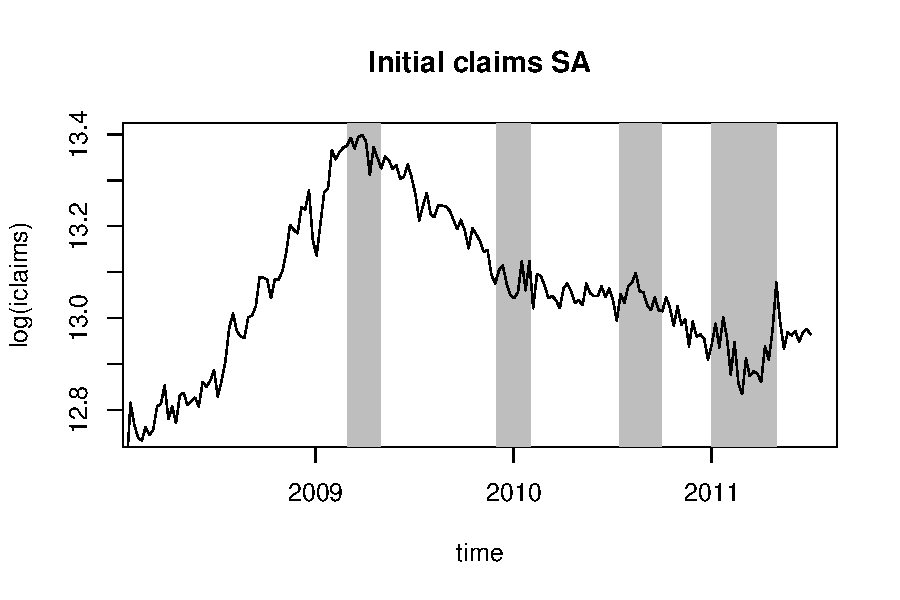
\includegraphics[width=5.5in]{iclaims}
\caption{\label{Fig:iclaims} Seasonally adjusted initial claims for unemployment; turning points in gray.} 
\end{center}
\end{figure}

Figure \ref{Fig:error} plots the difference in MAE for the Base and Trends
model.  A positive value indicates that the Trends forecast had a
smaller error.  Here it is clear that Trends model fits better during
the recession (December 2007 through June 2009), while the Base fits
better immediately after.


\begin{figure}[ht]
\begin{center}
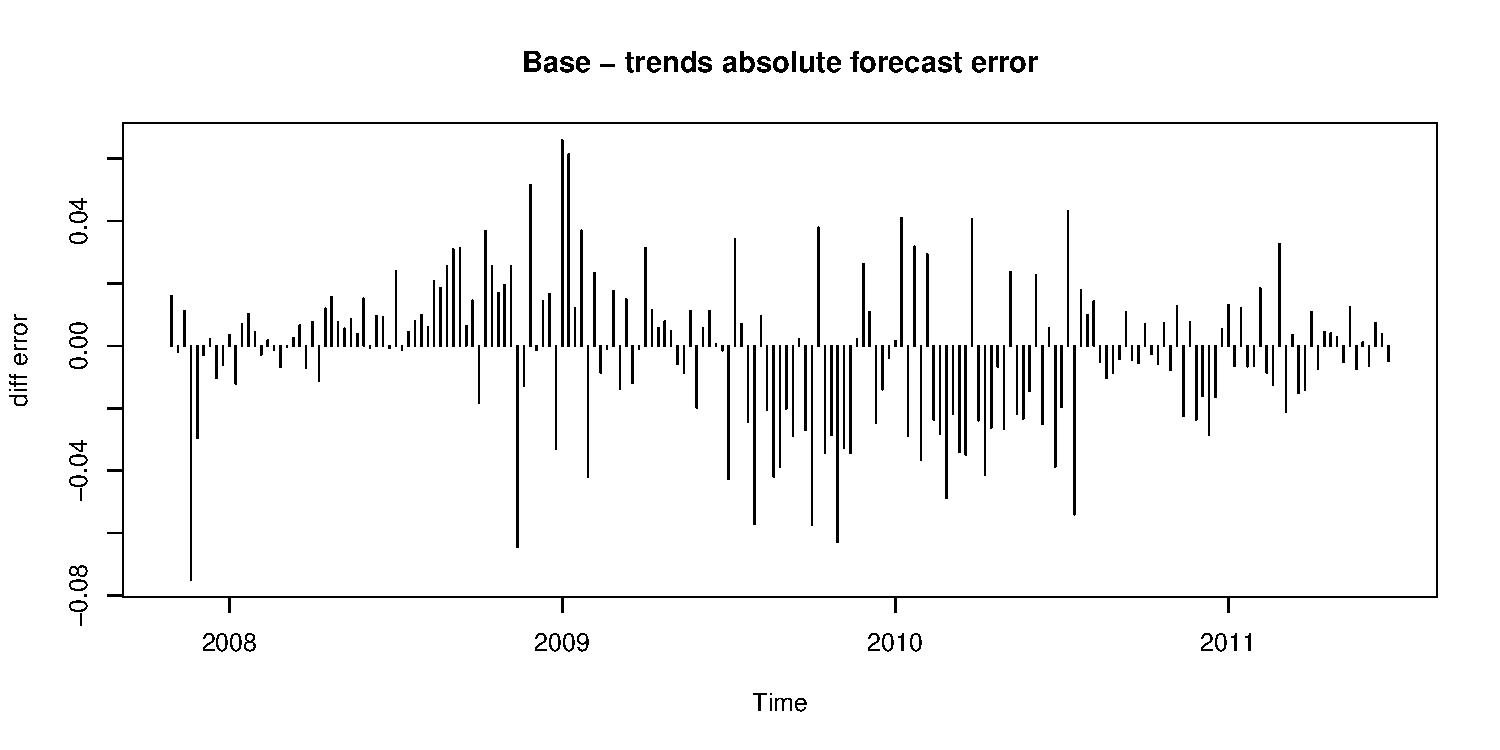
\includegraphics[width=5.5in]{error.pdf}
\caption{\label{Fig:error} Base absolute error -- Trends absolute error.} 
\end{center}
\end{figure}

\cite{Askitas10}, \cite{Suhoy09}, and \cite{Damuri10} have confirmed
the value of search data in forecasting unemployment in the U.S.,
Germany and Israel.

\subsection{Travel} 
The internet is commonly used for travel planning which suggests that
Google Trends data about destinations may be useful in predicting
visits to that destination.  We illustrate this using data from the
Hong Kong Tourism Board.\footnote{\url{http://partnernet.hktourismboard.com}}

The Hong Kong Tourism Board publishes monthly visitor arrival
statistics, including ``Monthly visitor arrival summary'' by
country/territory of residence. For this study we use visitor data
from US, Canada, Great Britain, Germany, France, Italy, Australia,
Japan and India.

``Hong Kong'' is also one of the subcategories in under Vacation
Destinations in Google Trends.  We can examine the query index for
this category by country of origin.

The Hong Kong visitor arrival data is not seasonally adjusted, nor is
the Google Trends data.  We used the average query index in the first
two weekly observations of the month to predict the total monthly
visitors.  Since the data is released with a one-month lag, this gives
us roughly a 6-week lead in terms of forecasting

We let $y_t$ be the visitors from a given country in month $t$, and
$x_t$ be the average Google Trends index for {\tt Vacation
  Destinations/Hong Kong} for the first two weeks of that month. We
can specify a basic seasonal AR-1 model of the form $y_t = b_1y_{t-1}
+ b_{12}y_{t-12} + b_0x_{t} + e_t$.

We estimate this model for each country and compare the actual to the
fitted results in Figure \ref{Fig:hk}.  Unlike the previous examples,
we have here used in-sample fits. As can be seen, the in-sample
fits are pretty good, with the exception of Japan.  Excluding Japan,
the average $R^2$ is 73.3\%.  In \cite{Choi09a} we use a more
elaborate random effects model with some additional predictors and
find a somewhat better in-sample fit.

\begin{figure}[ht]
\begin{center}
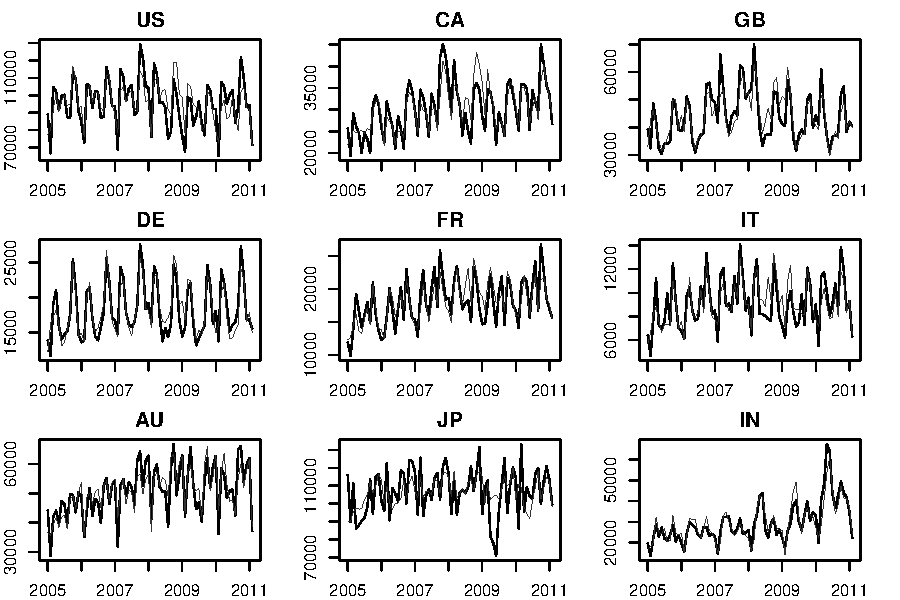
\includegraphics[width= 5.5in]{hk}
\caption{\label{Fig:hk} Visitors to Hong Kong} 
\end{center}
\end{figure}

\section{Consumer confidence \label{Sec:Confidence}}  

In our final example, we examine the Roy Morgan Consumer Confidence
Index for
Australia.\footnote{\url{http://www.roymorgan.com/news/polls/consumer-confidence.cfm}}
Unlike our earlier examples, it is not obvious what categories would
be most helpful in predicting this series.  There are a variety of
methods one can use for variable selection; see \cite{Castle10} for a
recent discussion of this topic with emphasis on nowcasting
applications.

We used a Bayesian method known as ``spike and slab'' regression first
described by \cite{George97}. This technique produces a posterior
probability that a variable enters a regression (i.e., has a non-zero
coefficient) along with an estimate of that coefficient's posterior
distribution.

We used Google Trends category data for Australia, taking the average
value of the category data for the first two weeks of the month and
seasonally adjusting it using the {\tt R} command {\tt stl}.  The
spike and slab technique assigned high posterior probabilities to the
categories {\tt Crime \& Justice}, {\tt Trucks \& SUVs}, and {\tt
  Hybrid \& Alternative Vehicles}.  The last two are not surprising as
they are highly correlated with the price of gasoline, which is known
to impact consumer confidence in the United States.  We have no
explanation for the first predictor. Plotting the {\tt Crime \&
  Justice} time series shows a definite correlation with consumer
confidence for the period we examine, but of course there is no way to
know if this correlation will persist in the future.

Our predictor for Australian log(consumer confidence) is summarized in
this table.

%\begin{framed}
\small
\begin{verbatim}
                                  Estimate Std. Error t value Pr(>|t|)    
  (Intercept)                    1.5172617  0.2795356   5.428 5.67e-07 ***
  lag(y, -1)                     0.6839436  0.0584158  11.708  < 2e-16 ***
  Crime...Justice               -0.0009664  0.0002404  -4.020 0.000129 ***
  Trucks...SUVs                  0.0010600  0.0005346   1.983 0.050735 .  
  Hybrid...Alternative.Vehicles -0.0007869  0.0001482  -5.308 9.26e-07 ***
  ---
  Multiple R-squared: 0.8583,	Adjusted R-squared: 0.8514 
\end{verbatim}
%\end{framed}
\normalsize

The Trends predictors reduce MAE of the simple AR-1 model by about
12.7\% for in-sample forecasts.  One-step-ahead MAE goes from 3.63\%
to 3.29\%, an improvement of 9.3\%; see Figure \ref{Fig:conf}.  The
big drop in Spring 2008 is due to a significant increase in queries on
{\tt Hybrid \& Alternative Vehicles} which is likely due to the
increased price of oil that occurred during that period.

\begin{figure}[ht]
\begin{center}
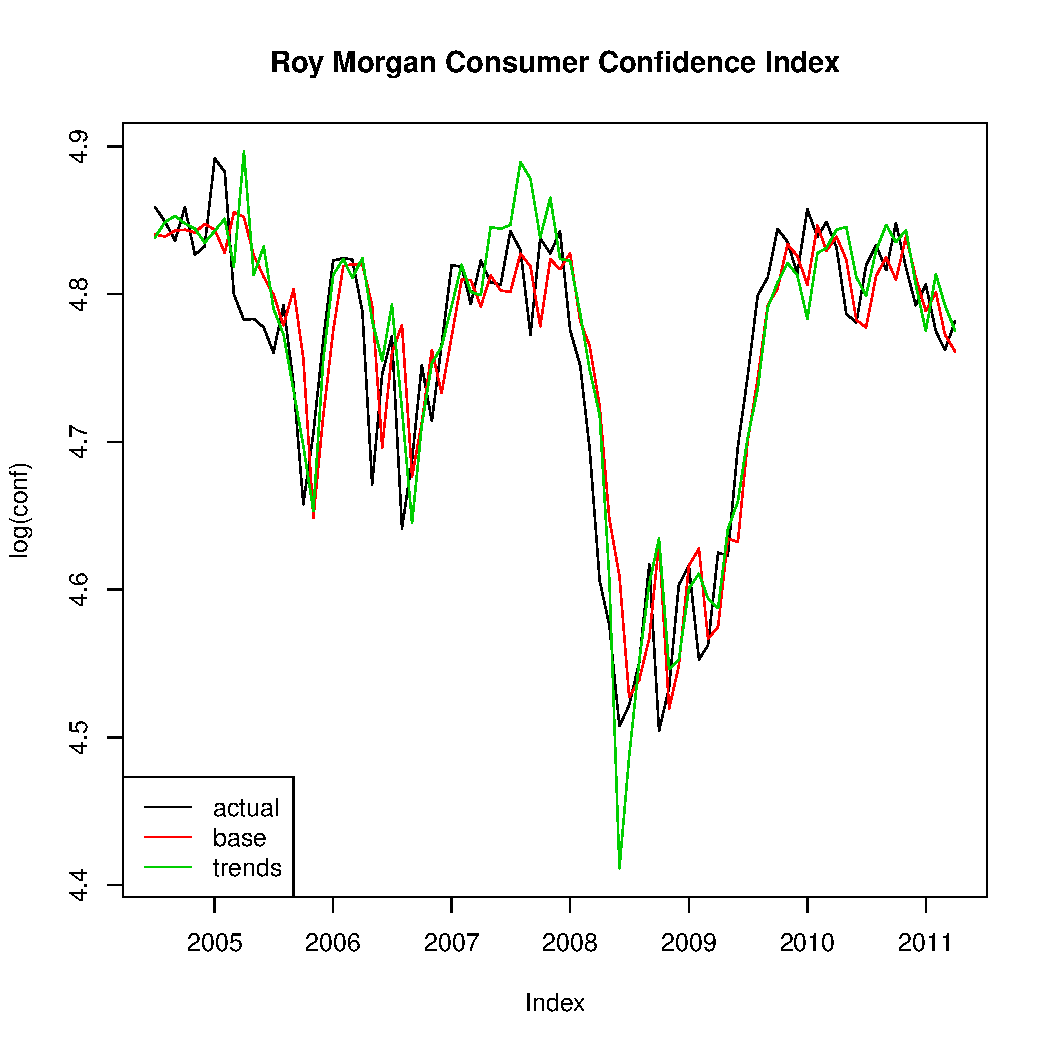
\includegraphics[width= 5.5in]{conf}
\caption{\label{Fig:conf} Australia consumer confidence.} 
\end{center}
\end{figure}

\section{Conclusion \label{Sec:Conclusion}}  

We have found that simple seasonal AR models that include relevant
Google Trends variables tend to outperform models that exclude these
predictors by 5\% to 20\%.  We hope that these examples will encourage
other researchers to experiment this data source in their own
research.

Google Trends data is available at a state and metro level for several
countries.  We have also had success with forecasting various business
metrics using state-level data.  It some cases longitudinal data helps
make up for the rather short time series available from Google Trends.

\newpage

\bibliographystyle{plainnat}
\bibliography{i4s}

\end{document}
